\begin{center}
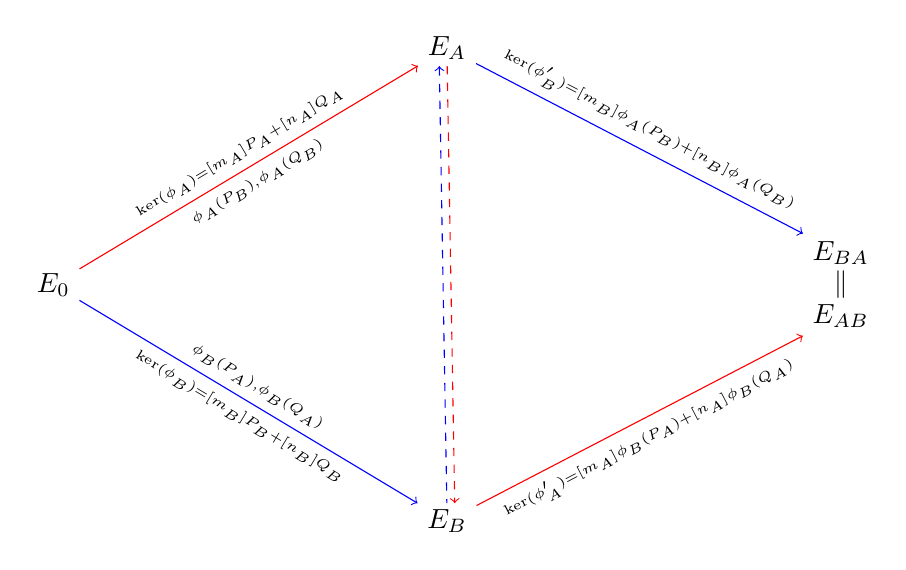
\begin{tikzpicture}
\node (1) at (-5cm,0cm){$E_0$};

\node (2) at (0cm,3cm){$E_A$};
\draw [color = red, ->] (1) -- (2);
\path (1) -- (2) node [above,sloped,pos=0.5]{$\scriptscriptstyle\ker(\phi_A)=\cyc{[m_A]P_A+[n_A]Q_A}$};
\path (1) -- (2) node [below,sloped,pos=0.5]{$\scriptscriptstyle\phi_A(P_B),\phi_A(Q_B)$};

\node (3) at (0cm,-3cm){$E_B$};
\draw [color = blue, ->] (1) -- (3);
\path (1) -- (3) node [below,sloped,pos=0.5]{$\scriptscriptstyle\ker(\phi_B)=\cyc{[m_B]P_B+[n_B]Q_B}$};
\path (1) -- (3) node [above,sloped,pos=0.5]{$\scriptscriptstyle\phi_B(P_A),\phi_B(Q_A)$};

\node (2a) at (0cm,2.9cm){};
\node (2b) at (-.1cm,2.9cm){};

\node (3a) at (.1cm,-2.9cm){};
\node (3b) at (0cm,-2.9cm){};

\draw [color = red, dashed, ->] (2a) -- (3a);
\draw [color = blue, dashed, <-] (2b) -- (3b);

\node (4) at (5cm,-.4cm){$E_{AB}$};
\draw [color = red, ->] (3) -- (4);
\path (3) -- (4) node [below,sloped,pos=0.5]{$\scriptscriptstyle\ker(\phi_A')=\cyc{[m_A]\phi_B(P_A)+[n_A]\phi_B(Q_A)}$};

\node (5) at (5cm,.4cm){$E_{BA}$};
\draw [color = blue, ->] (2) -- (5);
\path (2) -- (5) node [above,sloped,pos=0.5]{$\scriptscriptstyle\ker(\phi_B')=\cyc{[m_B]\phi_A(P_B)+[n_B]\phi_A(Q_B)}$};

\node (6) at (5cm,0cm){$\|$};

\end{tikzpicture}
\end{center}



